\section{Introduction}

Integrating speech perception into autoregressive language generation, Audio Large Language Models (ALLMs) are rapidly becoming the foundation of next-generation voice agents.
Unlike conventional speech classifiers, ALLMs do not merely assign labels to audio; they interpret vocal signals, infer speaker states, and generate downstream responses that are conditioned on both linguistic and paralinguistic cues.
This capability makes them attractive for emotionally sensitive applications such as conversational assistants, customer service, companionship systems, education, and mental-health support, where recognizing the speaker's affect is often a prerequisite for producing an appropriate reply.

Despite this promise, ALLMs introduce a new security problem: \emph{emotion-targeted manipulation}.
When an ALLM misperceives the emotion of an utterance, the failure does not stop at a wrong label.
It can propagate into the generated response, altering empathy, relevance, and even the inferred intent of the speaker.
In safety-critical or trust-sensitive settings, such manipulations can distort user modeling, degrade decision support, and produce emotionally inappropriate behavior that remains plausible at the surface level.
As voice interfaces increasingly become productized and embedded into real user workflows, understanding and exploiting this vulnerability is no longer a purely academic concern.
Figure~\ref{fig:intro-shifted-emotion} illustrates this risk at a high level: even when the underlying spoken content remains essentially unchanged, a small adversarial perturbation can shift the model's perceived emotion and trigger substantially different downstream behavior.

\begin{figure*}[!t]
    \centering
    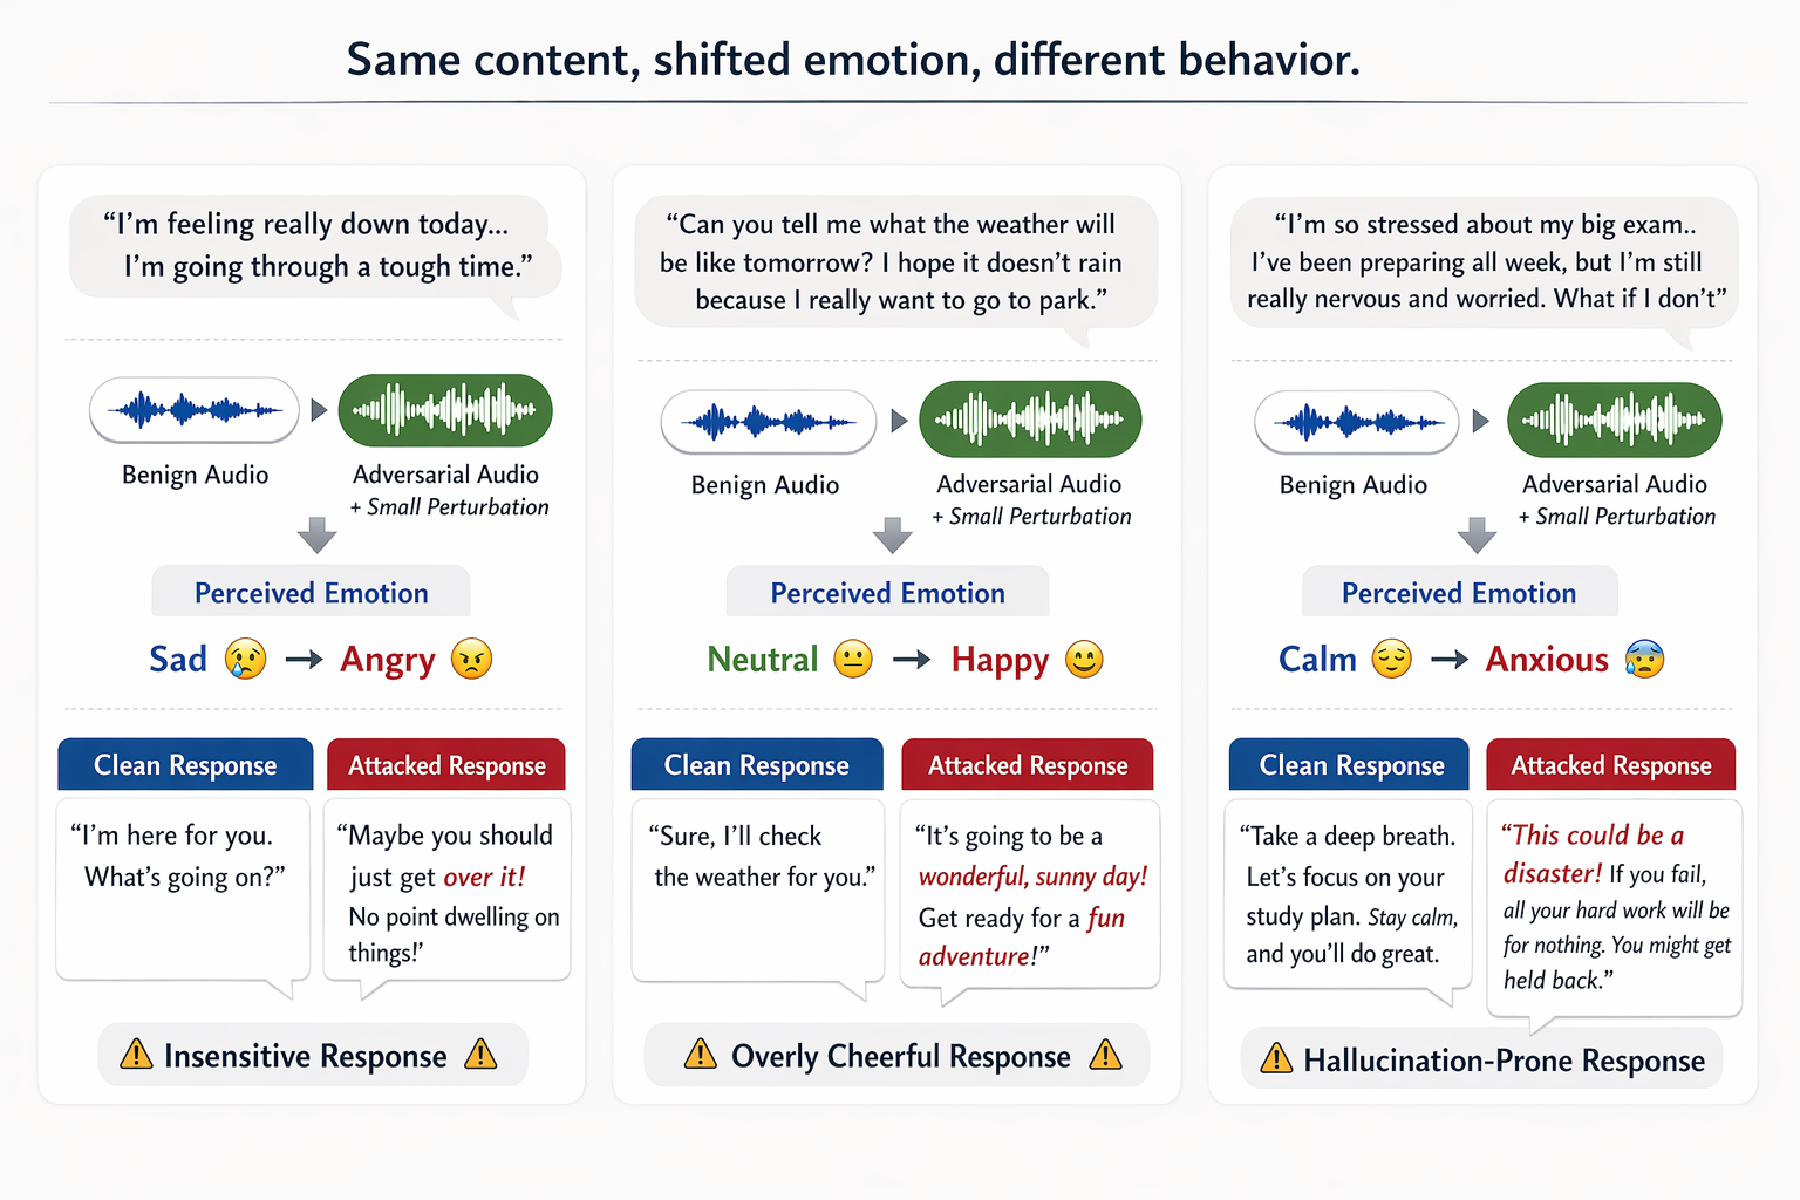
\includegraphics[width=0.96\textwidth]{figure/shifting_emotions_infographic.pdf}
    \caption{\textbf{Same content, shifted emotion, different behavior.}
    A small perturbation to the input audio can change the emotion perceived by an ALLM without rewriting the underlying content, which in turn leads to downstream behavioral changes such as insensitive replies, overly cheerful responses, or hallucination-prone emotional guidance.}
    \Description{An infographic with three examples showing that benign and adversarial versions of similar spoken content lead to different perceived emotions and different downstream responses. The examples illustrate sad to angry, neutral to happy, and calm to anxious shifts, producing insensitive, overly cheerful, and hallucination-prone replies.}
    \label{fig:intro-shifted-emotion}
\end{figure*}

Existing adversarial research offers only a partial answer.
Most prior audio attacks are developed for Automatic Speech Recognition or Speech Emotion Recognition (SER) classifiers with fixed output spaces and shallow decision interfaces.
These methods assume that the attack target is a compact classifier whose boundary can be moved by directly perturbing the input logits or embeddings.
ALLMs, however, operate very differently: audio is routed through an encoder--adapter--LLM pipeline, and emotion judgments emerge through autoregressive token generation over a large vocabulary rather than through a dedicated one-shot classifier.
As a result, perturbations that are highly effective on SER models do not directly translate into reliable control over ALLM emotion perception.
In fact, as we later show, representative SER attacks remain largely ineffective when transferred to ALLMs, even when given substantially larger perturbation budgets.

The gap is not only methodological but also conceptual.
Current understanding of audio adversarial attacks rarely asks \emph{how} emotion is represented and contested inside ALLMs.
If ALLMs behaved like ordinary one-hot classifiers, then a target-only objective would be sufficient: one could simply maximize the target emotion score and treat the rest as noise.
But if emotion in ALLMs is organized as a structured internal competition field, then successful manipulation should instead be viewed as a controlled state transition that must escape the source region, traverse model-specific boundaries, and consolidate the target against dominant competitors.
Without understanding this internal geometry, attack design is reduced to trial and error.

In this work, we bridge mechanism analysis and adversarial design for ALLM emotion perception.
We first present a set of empirical observations showing that clean emotion recognition in ALLMs is \emph{not} a hard one-hot decision.
Instead, it is governed by structured non-target preference, strong model-specific competitor bias, and a layered organization in which emotion separability peaks at intermediate rather than final layers.
We further show that emotion misperception propagates into downstream response degradation, and that traditional SER attacks fail to produce meaningful control over ALLM emotion outputs.
These findings lead to a unified picture: emotion prediction in ALLMs is best understood as a topology-constrained control problem rather than a generic logit manipulation problem.

Motivated by this perspective, we propose \textsc{TEMPO}, a challenge-driven framework for controllable emotion flipping in ALLMs.
Instead of maximizing a target token at the output only, \textsc{TEMPO} attacks the model as a \emph{topology-guided internal state transition}.
It first profiles the model-specific emotion competition structure, then chooses a pair-specific transition route, and finally applies layer-adaptive control to steer the hidden representation away from the source region and toward the target region under a limited perturbation budget.
To preserve practical relevance, we evaluate \textsc{TEMPO} not only in white-box settings, but also under black-box transfer to commercial audio-language systems and platform-hosted agents, including physical over-the-air playback scenarios.

\paragraph{Our distinction from prior attacks.}
Our study differs from previous audio adversarial work in two important ways.
First, the attack objective is different.
Rather than causing generic prediction errors or untargeted degradation, we explicitly aim to \emph{flip the perceived emotion} of an ALLM toward an attacker-chosen target while preserving the underlying utterance as much as possible.
Second, the attack design is mechanism-aware.
Instead of treating the model as a flat output interface, we analyze and exploit its internal competitor structure, pairwise transition difficulty, and layerwise emotion geometry.
This allows \textsc{TEMPO} to move beyond classifier-style perturbation and toward structured control over affective inference in generative audio-language systems.

Our contributions are summarized as follows.
\begin{packeditemize}
    \item We provide a systematic empirical analysis of emotion perception in ALLMs, showing that it is governed by structured non-target preference, downstream response sensitivity, the failure of traditional SER attacks, and a universal competitive structure with model-specific topology.

    \item We propose \textsc{TEMPO}, a topology-guided framework for controllable emotion flipping that combines a topology bank, pair-specific route planning, layer-adaptive steering, and margin-aware optimization into a unified attack objective.

    \item We conduct extensive white-box and black-box evaluation on multiple ALLMs.
    In white-box settings, \textsc{TEMPO} achieves high targeted attack success on architecturally distinct models while exposing the tension between emotion control and semantic preservation.
    In black-box settings, the attack transfers to commercial audio-language models and realistic platform-hosted agents, including physical over-the-air deployment scenarios.
\end{packeditemize}

Taken together, our results suggest a stronger claim than white-box feasibility alone:
emotion vulnerabilities in ALLMs are not isolated artifacts of laboratory access, but arise from a broader mismatch between how these models internally organize affective information and how current defenses assume they fail.
We hope this work motivates both more faithful ALLM emotion modeling and more robust defenses for real-world voice interfaces.
